\documentclass[dvipdfmx]{jsarticle}

\usepackage{listings}
\usepackage[dvipdfmx]{hyperref}
\usepackage{pxjahyper}
\usepackage{amsmath}
\usepackage{graphicx}
\usepackage{float}

\begin{document}

\lstset{
    frame=single,
    numbers=left
}

\title{アルゴリズムとデータ構造B グループワーク 報告書}
\author{水本 幸希}
\maketitle

\section{メンバー}
\begin{itemize}
  \item 水本 幸希
  \item 山口 慧
  \item 杣谷 星音
  \item 斧田 洋人
  \item 杉山 亮太
\end{itemize}

\section{基本的な考え方}
与えられたクエリと放送局のデータを切り取ったもの比較して、編集距離が最短となった放送局を答えとする。

\section{編集距離の求め方}

編集距離を求める方法には様々なものが存在するが、今回はビットパラレル法を採用した。
ビットパラレル法は動的計画法を応用しており、ビット演算を利用することで並列処理を行うことで計算時間を短縮している。
動的計画法の場合、計算量は$O(N^2)$であるが、ビットパラレル法を用いると$O(N)$まで計算量を減らすことができる。ただし、この計算量にするには配列の要素数が演算に使用するビット長と同じかそれ以下でなければならない。C言語の場合、使用できる変数の最大ビット長は64ビットであるからクエリの長さが65文字以上だとそのまま適用することができない。そのため今回はクエリの65文字目以降を捨てることで解決させた。これはクエリの長さが長いほど正答率が高くなり、64文字あればほぼ確実に正解を出せるためである。

\subsection{各アルゴリズムでの計測時間の比較}
以下に、様々な方法での実行時間を掲載する。なお、動的計画法での実行時間を100としている。各アルゴリズムの詳細については割愛する。

\begin{table}[H]
  \centering
  \begin{tabular}{c|c|c|c}
    動的計画法 & O(ND)アルゴリズム & O(NP)アルゴリズム & ビットパラレル法 \\ \hline\hline
    100 & 65.39 & 25.33 & 1.965 \\ \hline
  \end{tabular}
  \caption{各アルゴリズムでの実行時間}
\end{table}

このように、ビットパラレル法が最も効率良く計算できることが分かる。なお、O(NP)アルゴリズムと64文字で打ち切ったビットパラレル法のスコアを比較すると次のようになった。なお、本番で使用したプログラムにO(NP)アルゴリズムを組み込むと制限時間内に終わらないので、精度を粗くして計測した。(スコアは5個の平均値)

\begin{table}[H]
  \centering
  \begin{tabular}{c|c}
    O(NP)アルゴリズム & ビットパラレル法 \\ \hline\hline
    9749 & 9702 \\ \hline
  \end{tabular}
  \caption{文字の切り取りによる精度の違い}
\end{table}

このように、64文字あればほぼ問題なく答えを当てられるが、少し精度が落ちる。今回スコアを極限まで上げることができなかったのは64文字だけで判定したことことが原因だったと考えられる。

\section{放送局の信号分割と打ち切りの条件}

信号をクエリの長さだけ切り取る、ということを全ての箇所で行えば理論上かなり高い確率で当てることができる。ただし、切り取った開始位置の候補は、50万個存在しこれを全て走査してしまうと10秒以内には終わるが時間がかかりすぎてポイントに影響してくる。そのため、ある程度走査は粗くする必要性が生じる。以下に走査の幅とスコアの関係について、表と図で示す。変化が分かりやすいよう、高いスコアの出しにくいエラー率高めのケースで確認を行った。

\begin{table}[H]
  \centering
  \begin{tabular}{c|c|c}
    走査のステップ(クエリ長/N) & スコア & 実行時間[Sec] \\ \hline\hline
    1.0 & 3375 & 0.159 \\ \hline
    2.0 & 5345 & 0.323 \\ \hline
    3.0 & 7165 & 0.438 \\ \hline
    4.0 & 8470 & 0.605 \\ \hline
    5.0 & 8360 & 0.719 \\ \hline
    6.0 & 8395 & 0.879 \\ \hline
    7.0 & 8785 & 1.005 \\ \hline
    8.0 & 8815 & 1.108 \\ \hline
    9.0 & 8815 & 1.296 \\ \hline
    10.0 & 8985 & 1.453 \\ \hline
    15.0 & 9225 & 2.328 \\ \hline
    20.0 & 9280 & 3.248 \\ \hline
    走査幅=1 & 9175 & 6.708 \\ \hline
  \end{tabular}
  \caption{走査幅とスコアの関係}
\end{table}

\begin{figure}[H]
  \centering
  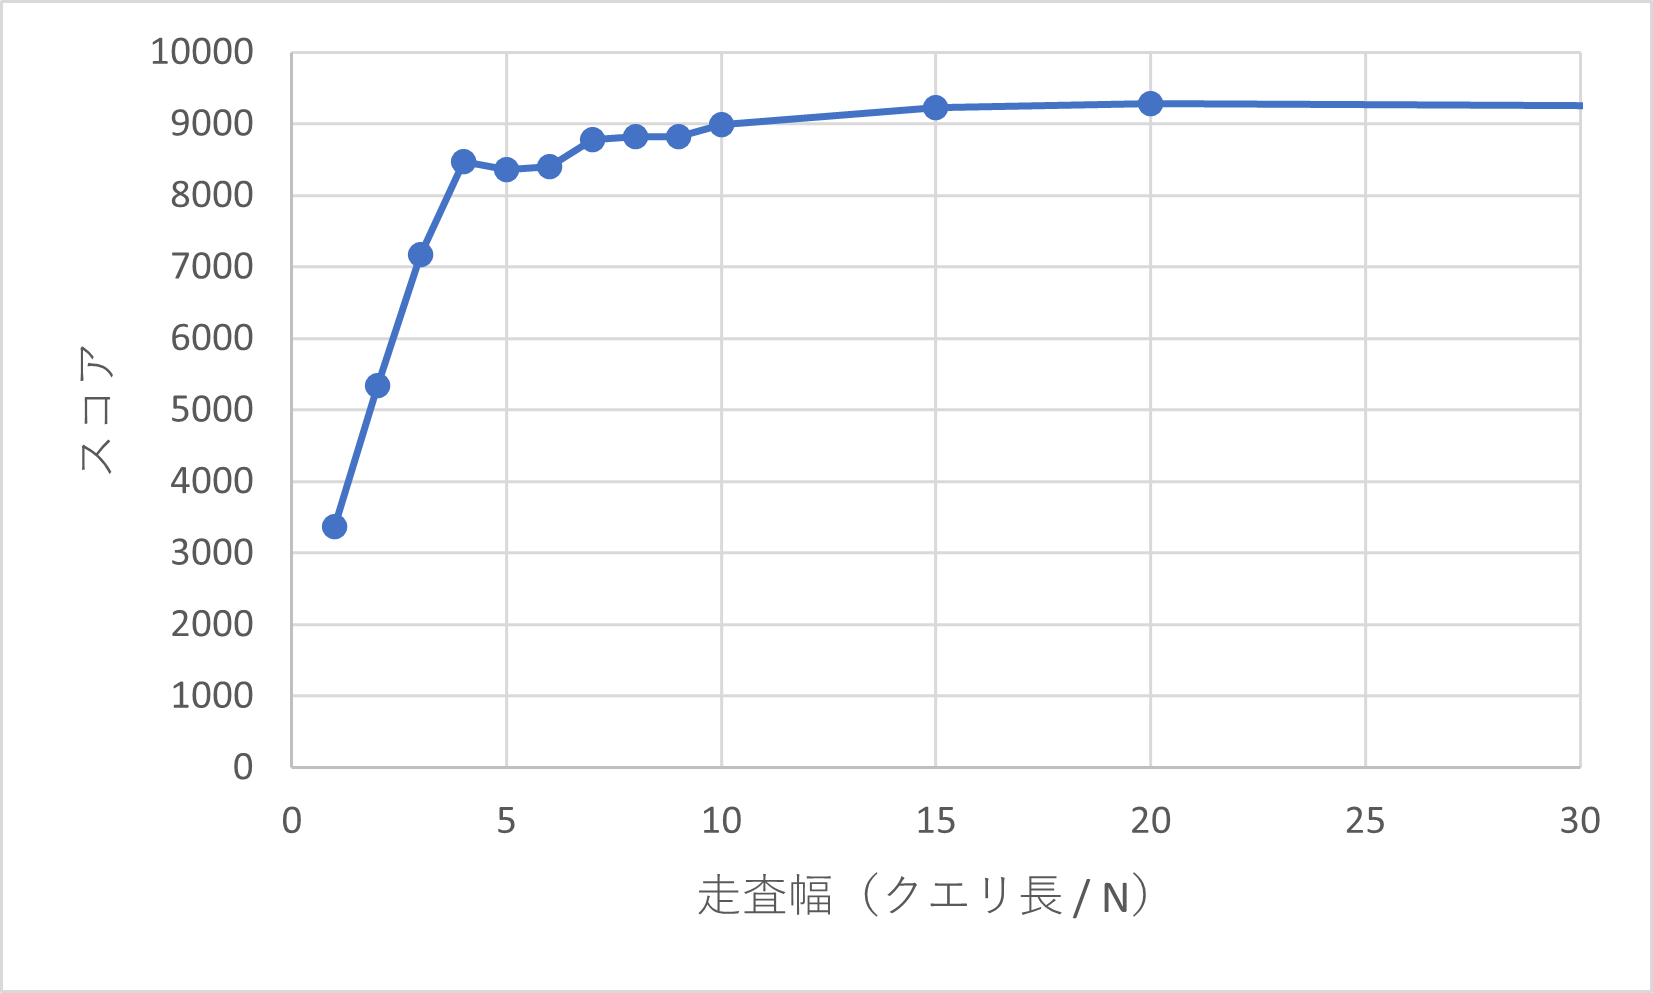
\includegraphics[scale = 1.0]{step.png}
  \caption{走査幅とスコアの関係}
\end{figure}

今回は、放送局の持つ信号からクエリの長さ分だけ信号を切り取って(最初は当然放送局の最初の位置から)編集距離を調べた後、放送局から切り取った信号の開始地点から$(クエリの長さ)/10$だけ右に移動し、再度編集距離を求める、といったことを繰り返すということを繰り返した。この場合、切り取った部分を走査するときは最大で$1/20$ずれる可能性がある。しかし、これ以上細かく走査してもスコアはあまり上がらず、逆に粗くすると正答率が低くなったので、走査するときのステップはこのように設定した。

また、これだけでも十分時間内に答えを求めることができるが、編集距離が著しく低いものが発見されたらその時点で答えを確定させて打ち切ってしまえば、正答率を下げることなく必要な時間をさらに短縮することができるその閾値の設定も色々試すことで決定した。以下に実験してみた結果を示す。この実験結果もエラー率が高い状態を想定している。

\begin{table}[H]
  \centering
  \begin{tabular}{c|c|c|c}
    打ち切りの閾値(クエリ長/N) & スコア & 打ち切った回数 & 実行時間[Sec] \\ \hline\hline
    1.0 & 0 & 100 & 0.009 \\ \hline
    2.0 & 1800 & 100 & 0.233 \\ \hline
    3.0 & 7750 & 77 & 1.055 \\ \hline
    3.5 & 8800 & 54 & 1.271 \\ \hline
    4.0 & 9100 & 33 & 1.448 \\ \hline
    5.0 & 8800 & 12 & 1.627 \\ \hline
    6.0 & 8955 & 4 & 1.642 \\ \hline
    7.0 & 8970 & 1 & 1.651 \\ \hline
    8.0 & 9100 & 0 & 1.700 \\ \hline
    9.0 & 8815 & 0 & 1.703 \\ \hline
    10.0 & 8860 & 0 & 1.714 \\ \hline
    打ち切りなし & 8970 & 0 & 1.719 \\ \hline
  \end{tabular}
  \caption{打ち切りの閾値とスコアの関係}
\end{table}

\begin{figure}[H]
  \centering
  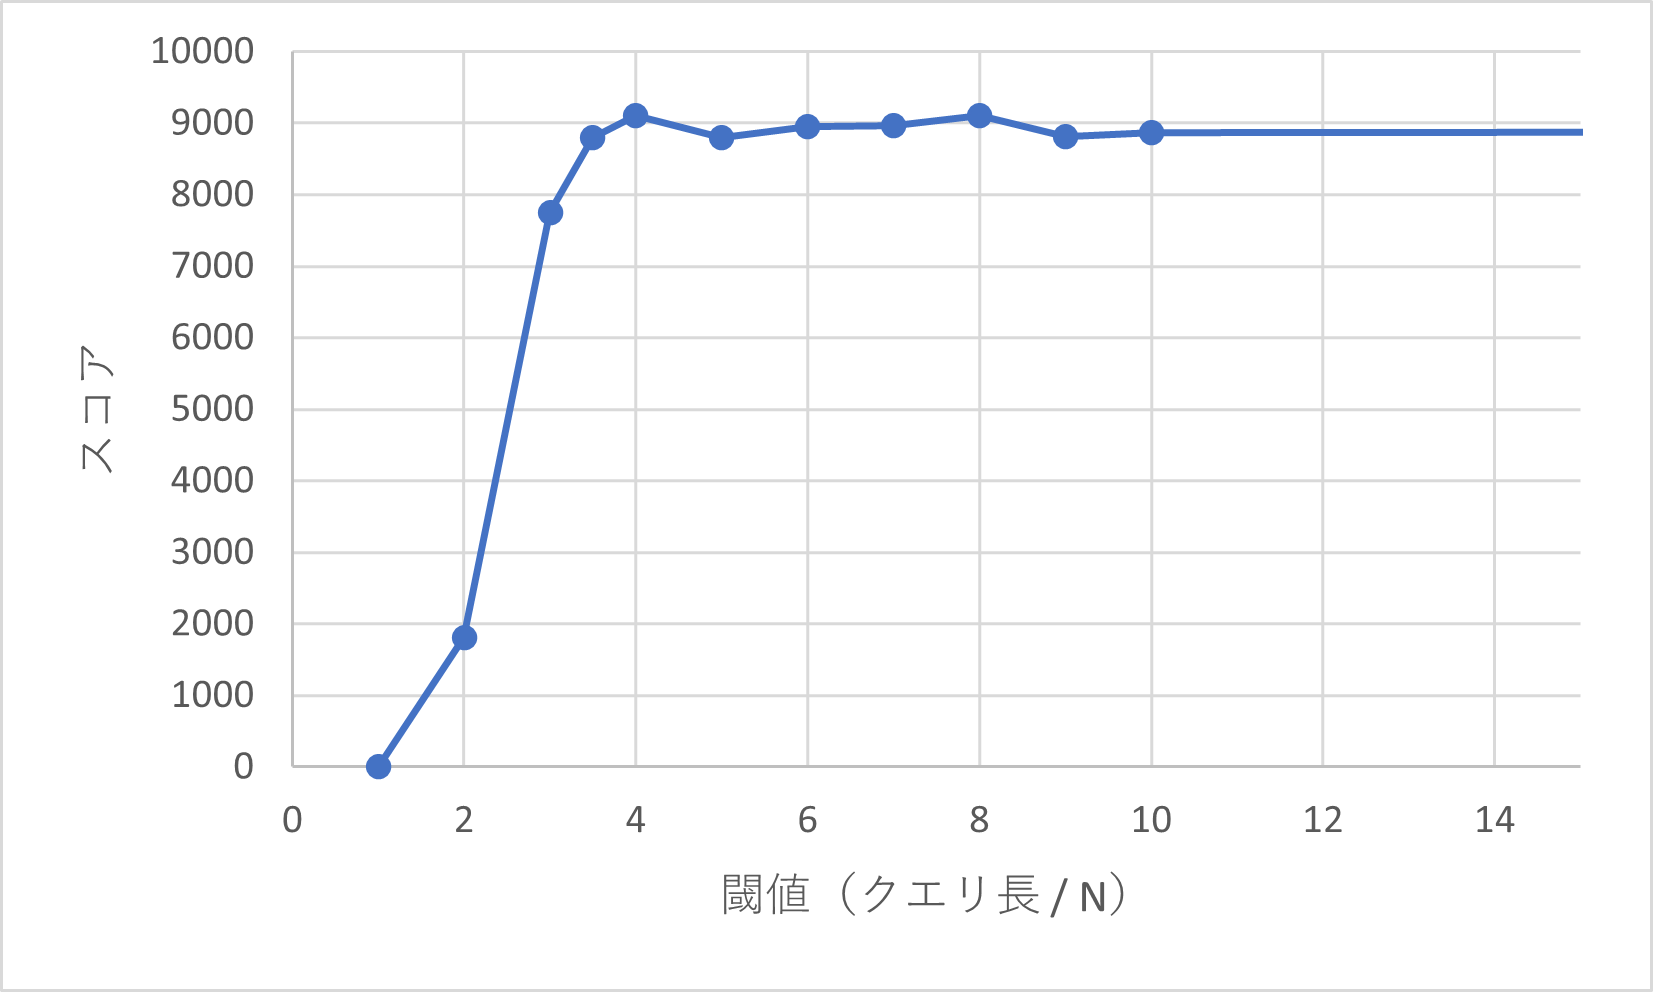
\includegraphics[scale = 1.0]{filter.png}
  \caption{打ち切りの閾値とスコアの関係}
\end{figure}

今回は、編集距離がクエリの長さの$1/4$以下になった場合はその場で打ち切った。これ以上小さくしても結果は変わらず逆に大きくすると、間違える可能性が増加したためである。なお、発表を聞いて編集距離の打ち切りに関しては信頼区間内に収まっているかどうかで判断すればよいということを新しく知った。今回は手探りでパラメータを指定したが、今後は手探りだけではなく論理的に設定することが重要だと感じた。

\section{クエリを聞き直す条件}

これまでの工夫で、それなりに正解を出すことができるが信号が短い場合の正答率が低くなってしまう。これは各放送局での最短編集距離が最も小さい放送局が複数存在する場合、最初に発見した放送局を答えとしてしまうようなプログラムにしたことが原因であった。これを解決するため、最短編集距離が最も短いものが複数存在する場合はクエリを聞き直し、それらの放送局に対して最短編集距離を再度求めることで、放送局を確定させた。これによってさらに正答率を上昇させることができた。一方、最短編集距離と差が1しかない場合も聞き直してみたが、精度が上がらないどころが時間内に終わらせることができなかったので却下となった。

\section{苦戦したところ}

今回ビットパラレル法を用いた手法を提案した。この手法では挿入、削除コストは1、置換コストは2となっている(置換は考慮されず、挿入と削除を組み合わせて計算しているため)。色々試したところ、今回の条件では置換コストを2とした方が確実に正答率が上昇したため置換コストは1とすることはしなかった。そのため、挿入、削除率が高い場合でも高いスコアを出すことができるが、置換率が高い状況では高いスコアを出すことが難しかった。特に、クエリの長さが短い場合は正答を出すことが困難であり今回はそれらのケースで確実に正解を出すことは断念した。

\section{没となった案}
\begin{enumerate}
  \item メモリピークを抑えるために各データを2ビット(0, 1, 2, 3)に圧縮 \\
    → 制限時間内にプログラムが終わらなくなったので没
  \item クエリを聞き直したときにすでに聞いた信号と合わせてより正確な信号にする \\
    → やり方が分からなかったので没
  \item 何個かのクエリを用意してそれぞれの場合での編集距離の平均から最短編集距離を出す \\
    → 全くスコアが上がらなかったので没
\end{enumerate}

\section{結果}

以下に100個のテストケースで実行したときのスコアを記載する。(下の二つは最初に配布された10個のテストケースでの平均値)

\begin{itemize}
  \item スコア 968035
  \item 実行時間 1.24 [Sec]
  \item メモリピーク 2.209 [MB]
  \item クエリを聞き直した回数 9.7 回
  \item 編集距離が短いものを発見して中断した回数 62.7 回
\end{itemize}

答えを外したのは、クエリが短かったり、置換率が高い場合がほとんどであった。また、エラー率が高い状況では他班と比較して高いスコアが得られたが、逆にエラー率が低い条件では高いスコアを出すことができず、1位を取ることが出来なかった。これは、65文字目以降を捨てていることでわずかに精度が落ちていることが原因であると考えられる。

\section{まとめ}

\begin{itemize}
  \item ビットパラレル法を用いて各放送局の最短編集距離を求めるが、クエリの65文字目以降は使わずに予測する。
  \item 走査は1バイトずつではなく、1回につきクエリの長さの$1/10$だけ右に進めていく
  \item 編集距離が著しく短い(クエリの長さの$1/4$以下)場合はその時点で答えを確定させてそのクエリに対する走査は打ち切る
  \item 最短編集距離が複数で同一だった場合はクエリを聞き直して再度求めなおす
  \item 置換コストは2、挿入、削除コストを1とすると切り取った部分以外との編集距離を増やすため正確に答えを出せる
  \item 今回の手法では、「クエリが短い」、「置換率が高い」場合に正答率が低くなる
\end{itemize}

以下にフローチャートを示す。

\begin{figure}[H]
  \centering
  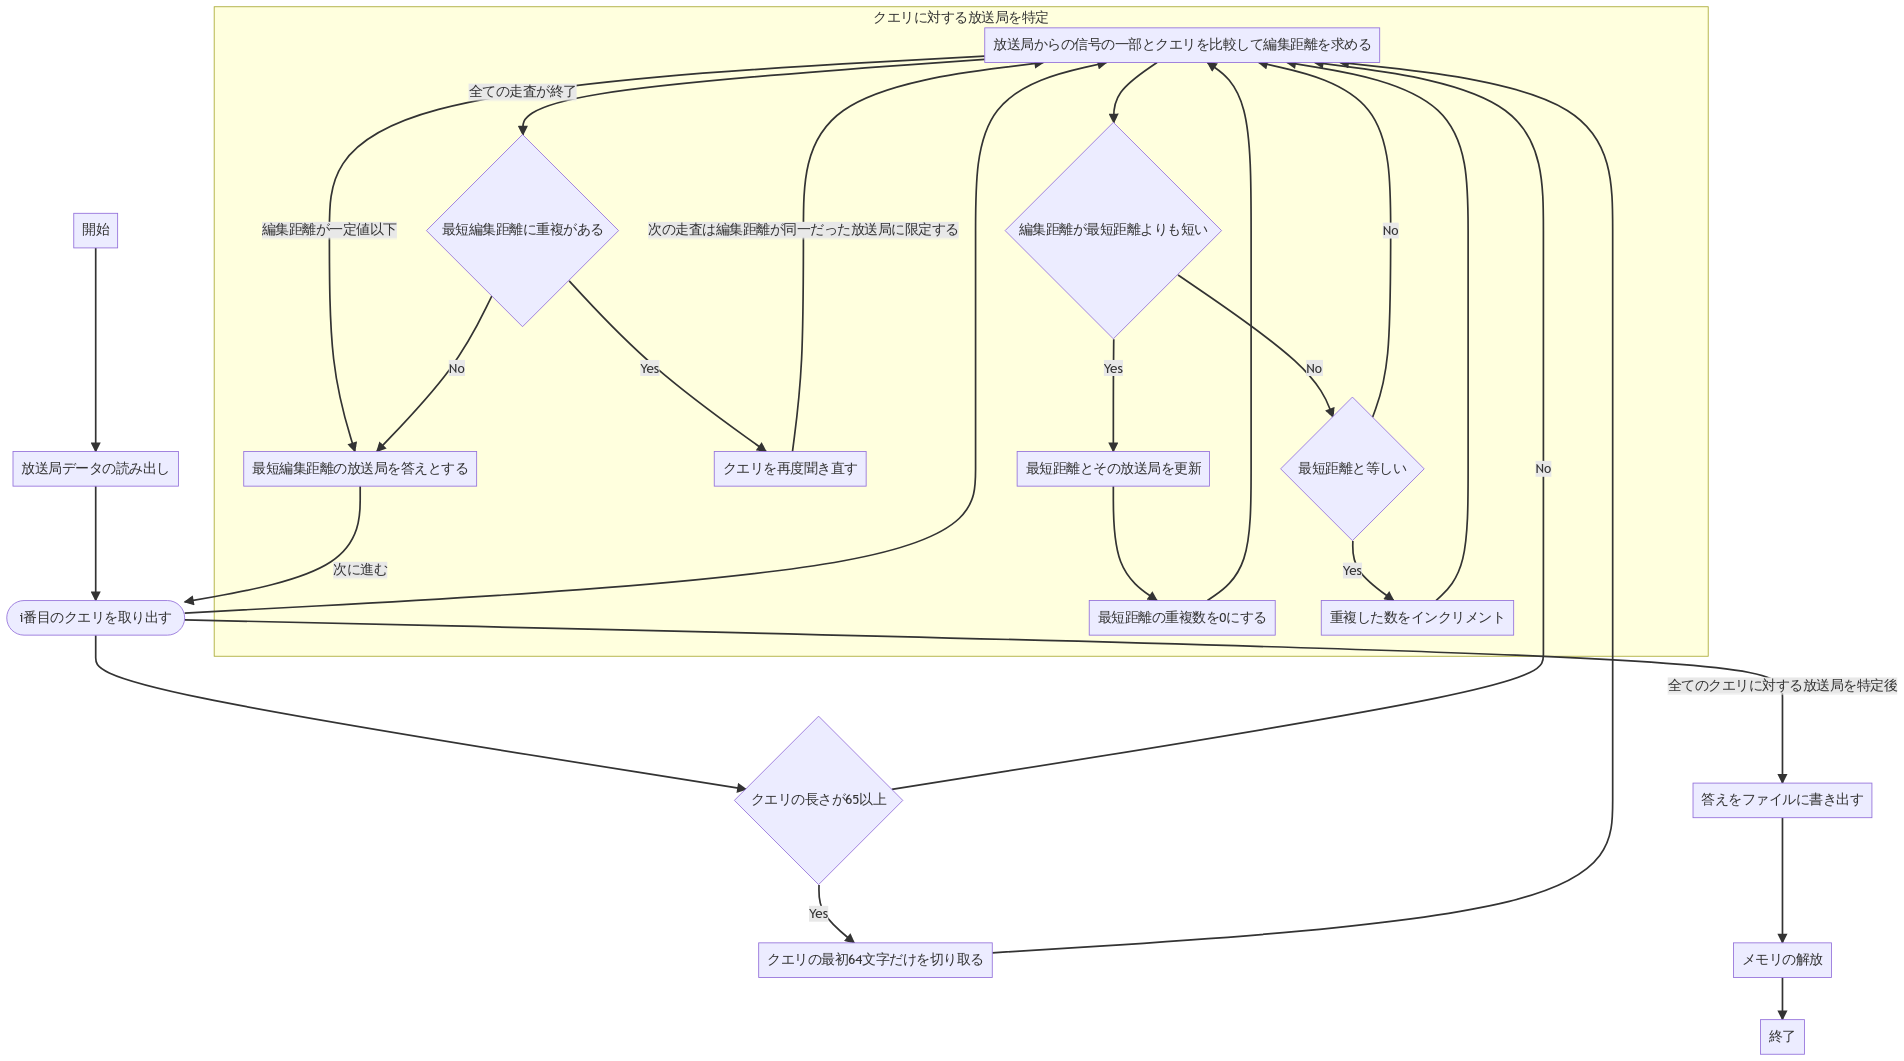
\includegraphics[scale = 0.25]{flowchart.png}
  \caption{実行フローチャート}
\end{figure}

\section{ソースコード}

以下に今回使用したソースコードを示す。マクロを定義することで、得点や時間が表示されるように設計した。

\begin{lstlisting}[language=C++]
// #define EVALUATE_MODE

#include <stdio.h>
#include <stdlib.h>
#include <string.h>
#ifdef EVALUATE_MODE
#include <time.h>
#endif

#include "ask.h"

#ifndef INT_MAX
#define INT_MAX 0x7fffffff
#endif

static int p_ins, p_sub, p_del;
static char **S;
static char *q;

#ifdef EVALUATE_MODE
static int abort_count = 0;
static int ask_count = 0;
static int compute_time;

void evaluate(char *argv[])
{
#pragma GCC diagnostic ignored "-Wunused-result"
	FILE *output_file = fopen(argv[2], "r");
	FILE *answer_file = fopen(argv[3], "r");

	int p_ins, p_sub, p_del;
	fscanf(answer_file, "%d %d %d", &p_ins, &p_sub, &p_del);

	int correct = 0, i;
	for (i = 0; i < N; i++)
	{
		int input[N], answer[N];
		char data[N];
		if (fscanf(output_file, "%d", &input[i]) == EOF)
			break;
		fscanf(answer_file, "%d %s", &answer[i], data);
		if (input[i] == answer[i])
			correct++;
	}

	printf("%d\n", correct * 100 - ask_count * 5);
	// printf("%d/%d Correct.\n", correct, i);
	// printf("Score: %d\n", correct * 100 - ask_count * 5);
	// printf("Time: %lf seconds\n", (double)compute_time / CLOCKS_PER_SEC);
	// printf("Ask count: %d\n", ask_count);
	// printf("Abort count: %d\n", abort_count);
	// printf("\n");

	fclose(output_file);
	fclose(answer_file);
#pragma GCC diagnostic warning "-Wunused-result"
}
#endif

#pragma region BITPARALLEL
int weighted_levenshtein_bitpal(char *a, char len_a, char *b, int len_b)
{
	if (len_a > 64)
	{
		return weighted_levenshtein_bitpal(a, 64, b, len_b > 64 ? 64 : len_b);
	}

	unsigned long long posbits[256] = {0};

	for (int i = 0; i < len_a; i++)
	{
		posbits[(unsigned char)a[i]] |= 1ull << i;
	}

	unsigned long long DHneg1 = ~0x0ull;
	unsigned long long DHzero = 0;
	unsigned long long DHpos1 = 0;

	// recursion
	for (int i = 0; i < len_b; i++)
	{
		unsigned long long Matches = posbits[(unsigned char)b[i]];
		// Complement Matches
		unsigned long long NotMatches = ~Matches;

		// Finding the vertical values.
		// Find 1s
		unsigned long long INITpos1s = DHneg1 & Matches;
		unsigned long long DVpos1shift = (((INITpos1s + DHneg1) ^ DHneg1) ^ INITpos1s);

		// set RemainingDHneg1
		unsigned long long RemainDHneg1 = DHneg1 ^ (DVpos1shift >> 1);
		// combine 1s and Matches
		unsigned long long DVpos1shiftorMatch = DVpos1shift | Matches;

		// Find 0s
		unsigned long long INITzeros = (DHzero & DVpos1shiftorMatch);
		unsigned long long DVzeroshift = ((INITzeros << 1) + RemainDHneg1) ^ RemainDHneg1;

		// Find -1s
		unsigned long long DVneg1shift = ~(DVpos1shift | DVzeroshift);
		DHzero &= NotMatches;
		// combine 1s and Matches
		unsigned long long DHpos1orMatch = DHpos1 | Matches;
		// Find 0s
		DHzero = (DVzeroshift & DHpos1orMatch) | (DVneg1shift & DHzero);
		// Find 1s
		DHpos1 = (DVneg1shift & DHpos1orMatch);
		// Find -1s
		DHneg1 = ~(DHzero | DHpos1);
	}
	// find scores in last row
	unsigned long long add1 = DHzero;
	unsigned long long add2 = DHpos1;

	int dist = len_b;

	for (int i = 0; i < len_a; i++)
	{
		unsigned long long bitmask = 1ull << i;
		dist -= ((add1 & bitmask) >> i) * 1 + ((add2 & bitmask) >> i) * 2 - 1;
	}

	return dist;
}
#pragma endregion

int predict_answer(const int index, char *answer_file, const int length, int *ids, const int k)
{
	int ans_id = -1;
	int min_distance = INT_MAX;
	int multiple = 0;
	int ans_ids[N] = {0};
	const int step = length / 10.0;
	for (int j = 0; j < k; j++)
	{
		int id = ids[j];
		for (int i = 0; i < DATA_LENGTH; i += step)
		{
			static char temp[N + 1];
			strncpy(temp, S[id] + i, length);
			temp[length] = '\0';
			int distance = weighted_levenshtein_bitpal(temp, length, q, length);
			if (distance < min_distance)
			{
				min_distance = distance;
				ans_id = id;
				multiple = 0;
				ans_ids[0] = id;
			}
			if (distance == min_distance && ans_id != id)
			{
				if (ans_ids[multiple] != id)
				{
					multiple++;
					ans_ids[multiple] = id;
				}
			}
			if (distance < length / 4.0)
			{
#ifdef EVALUATE_MODE
				abort_count++;
#endif
				return ans_id + 1;
			}
		}
	}
	if (multiple)
	{
		free(q);
#ifdef EVALUATE_MODE
		ask_count++;
#endif
		q = ask(index + 1, answer_file);
		return predict_answer(index, answer_file, strlen(q) + 1, ans_ids, multiple + 1);
	}
	return ans_id + 1;
}

int main(int argc, char *argv[])
{
#pragma GCC diagnostic ignored "-Wunused-result"
#pragma region INITIALIZE
#ifdef EVALUATE_MODE
	compute_time = clock();
#endif
	srand((unsigned int)time(NULL));
	FILE *input_file = fopen(argv[1], "r");
	FILE *output_file = fopen(argv[2], "w");
	FILE *answer_file = fopen(argv[3], "r");
	int ids[N];
	for (int i = 0; i < N; i++)
	{
		ids[i] = i;
	}

	if (!input_file || !output_file || !answer_file)
	{
		fprintf(stderr, "error\n");
		exit(EXIT_FAILURE);
	}

	fscanf(input_file, "%d %d %d", &p_ins, &p_sub, &p_del);

	S = (char **)malloc(sizeof(char *) * N);

	for (int i = 0; i < N; i++)
	{
		S[i] = (char *)malloc(sizeof(char) * (DATA_LENGTH + 1));
		fscanf(input_file, "%s", S[i]);
	}
#pragma endregion

	for (int i = 0; i < Q; i++)
	{
		q = malloc(sizeof(char) * (N + 1));
		fscanf(input_file, "%s", q);
		int length = strlen(q) + 1;

		int answer = predict_answer(i, argv[3], length, ids, N);
		free(q);

		fprintf(output_file, "%d\n", answer);
	}

#pragma region FINALIZE
	fclose(input_file);
	fprintf(output_file, "%lf\n", clock() / (double)CLOCKS_PER_SEC);
	fclose(output_file);
	fclose(answer_file);
	for (int i = 0; i < N; i++)
	{
		free(S[i]);
	}
	free(S);
#pragma endregion
#pragma GCC diagnostic warning "-Wunused-result"

#ifdef EVALUATE_MODE
	compute_time = clock() - compute_time;
	evaluate(argv);
#endif

	return 0;
}
\end{lstlisting}

また、提出したソースコードにはないが、時間の確認に使った動的計画法、O(ND)アルゴリズム、O(NP)アルゴリズムのソースコードについても以下に記載する。
\begin{lstlisting}[language=C++]
#define max(a,b) (((a) > (b)) ? (a) : (b))
#define min(a,b) (((a) < (b)) ? (a) : (b))

int edit_distance_dp(char *a, int len_a, char *b, int len_b)
{
    static int d[101][101];

    for (int i = 0; i < len_a + 1; i++) d[i][0] = i;
    for (int i = 0; i < len_b + 1; i++) d[0][i] = i;
    for (int i = 1; i < len_a + 1; i++)
        for (int j = 1; j < len_b + 1; j++)
            d[i][j] = min(min(d[i-1][j], d[i][j-1]) + 1, d[i-1][j-1] + (a[i-1] == b[j-1] ? 0 : 1));

    return d[len_a][len_b];
}

int edit_distance_ond(char *a, int len_a, char *b, int len_b)
{
    static int V[201];
    int x, y;
    int offset = len_a;
    V[offset + 1] = 0;

    for (int D = 0; D <= len_a + len_b; D++) {
        for (int k = -D; k <= D; k += 2) {
            if (k == -D || k != D && V[k-1+offset] < V[k+1+offset]) x = V[k+1+offset];
            else x = V[k-1+offset] + 1;
            y = x - k;
            while (x < len_a && y < len_a && a[x] == b[y]) {
                x++;
                y++;
            }
            V[k+offset] = x;
            if (x >=  len_a && y >= len_b) return D;
        }
    }

    return -1;
}

static int snake(int k, int y, char *a, int len_a, char *b, int len_b)
{
    int x = y - k;

    while (x < len_a && y < len_b && a[x] == b[y]) {
        x++;
        y++;
    }

    return y;
}

int edit_distance_onp(char *a, int len_a, char *b, int len_b)
{
    // required: s1->size() <= s2->size()
    char** s1 = len_a > len_b ? &b : &a;
    char** s2 = len_a > len_b ? &a : &b;
	const int s1_size = len_a > len_b ? len_b : len_a;
	const int s2_size = len_a > len_b ? len_a : len_b;
    static int fp[201];
    int x, y, k, p;
    int offset = s1_size + 1;
    int delta = s2_size - s1_size;
    for (int i = 0; i < 201; i++) fp[i] = -1;

    for (p = 0; fp[delta + offset] != s2_size; p++) {
        for(k = -p; k < delta; k++)
            fp[k + offset] = snake(k, max(fp[k-1+offset] + 1, fp[k+1+offset]), *s1, s1_size, *s2, s2_size);
        for(k = delta + p; k > delta; k--)
            fp[k + offset] = snake(k, max(fp[k-1+offset] + 1, fp[k+1+offset]), *s1, s1_size, *s2, s2_size);
        fp[delta + offset] = snake(delta, max(fp[delta-1+offset] + 1, fp[delta+1+offset]), *s1, s1_size, *s2, s2_size);
    }

    return delta + (p - 1) * 2;
}
\end{lstlisting}

\begin{thebibliography}{99}
  \item "bitparallel weighted Levenshtein distance". Stackoverflow. \url{https://stackoverflow.com/questions/65363769/bitparallel-weighted-levenshtein-distance} (参照 2022-1-25)
  \item "C++: 編集距離を求めるアルゴリズム". 良いもの。悪いもの。 \url{http://handasse.blogspot.com/2009/04/c_29.html} (参照 2022-1-25)
\end{thebibliography}

\end{document}